%! Author = adnansiddiquei
%! Date = 07/12/2023

\section{Development, Experimentation and Profiling}\label{sec:development-experimentation-and-profiling}
Here we discuss several components of the development process, and reason why we chose to do things in certain ways.

\subsection{Linting and Formatting - \inlinecode{ruff}}\label{subsec:linting-and-formatting}
    Linting and formatting is useful, especially in shared projects, as it allows for a consistent style across the codebase.
    There are a plethora of python linting and formatting tools available and for this project, we chose to use \inlinecode{ruff}.
    There were two primary reasons for this choice: speed and simplicity.
    \inlinecode{ruff} is faster than most other linting tools including \inlinecode{flake8}.
    In a test done by the developers of \inlinecode{ruff}, it managed to lint the CPython codebase 42x faster than
    \inlinecode{flake8} \cite{ruff-repo}.

    Additionally, \inlinecode{ruff} provides formatting functionality and as such it can also replace tools such as
    \inlinecode{black}.
    This makes the implementation of linting and formatting simpler, as we only need to use one tool.
    \inlinecode{ruff}'s configuration capabilities allow it to lint and format to any standard we want to, and therefore,
    it was configured to mimic \inlinecode{black} and \inlinecode{flake8}'s default config in accordance with PEP8.

    \subsection{Git and Gitlab Workflows}\label{subsec:git-and-gitlab-pipeline}
    It is generally good practise to write detailed commit messages and merge requests, and traditionally in larger
    software projects, project management tools such as JIRA are used to track issues and tasks, with merge requests
    being linked to these issues.
    In the world of open source, and small projects like this, GitLab's issue tracker works as a perfect tool for this.
    Therefore, we utilised the issue tracker to create issues for tasks that needed to be done, and then linked merge requests
    to these issues.
    In this way, we could maintain detailed documentation in the issue tracker of what was done, and why it was done,
    in a slightly more structured way than just using commit messages.
    Therefore, a new branch was created for every issue, and once the branch implemented or resolved the features in the
    issue, a merge request was created, linked to the issue, merged into main, and the issue was closed.
    As such, anyone with access to the repo can see the git commit history through the GitLab UI and any references to issue
    numbers in commits can be clicked to link the user to the underlying issue which describes what was implemented and why.

    Furthermore, a nice feature of many project management tools and IDE's is the ability to group branches into folders
    based on the branch name.
    Git allows forward slashes '/' in branch names such that branches can be structured into folders by the IDE, and so
    a naming convention was adopted for branches.
    Branches were named like the following: \inlinecode{feat/issue-1} or \inlinecode{tests/issue-4} where the 3 main
    'folders' used were \inlinecode{feat} for feature, \inlinecode{tests} and \inlinecode{bug}, followed by
    the issue number it implemented.
    In practise, the \inlinecode{bug} folder was not used as no bugs were discovered.

    Overall, these Git and GitLab workflows allowed for a structured development process, and a detailed history of
    what was done and why it was done, which is useful for future reference.

    \subsection{Test Driven Development}\label{subsec:test-driven-development}
    Where possible, we strived to do test driven development by writing tests first.
    This was made possible due to the careful prototyping and API design discussed in Section\eqref{sec:solution-design}.
    The reason we decided to write tests first came from three primary reasons:
    \begin{itemize}
        \item it streamlined code writing, as we were already aware of what the code needed to do, and what the edge cases
        were.
        \item it defined clearly what the end product would be;
        \item it reduced debugging time.
        We could more quickly figure out what was going wrong if a bug arose;
    \end{itemize}
    The final tests that were written are discussed more in Section\eqref{sec:validation-unit-tests-and-ci-set-up}.

    \subsection{Profiling and Optimisation}\label{subsec:profiling-and-optimisation}
    \begin{figure}[htb]
    \centering
    \begin{subfigure}[b]{0.9\linewidth}
        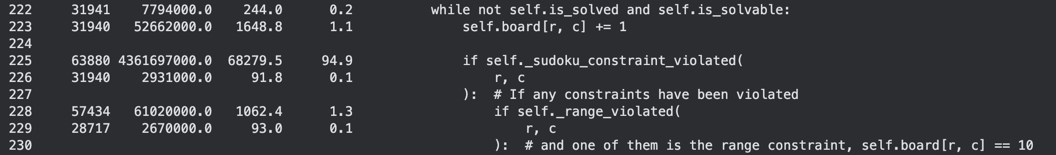
\includegraphics[width=\linewidth]{figures/line_profile1}
        \caption{An excerpt of the line profile of the \inlinecode{BacktrackingSolver.solve} function. Line 220 indicates
        the that the \inlinecode{BacktrackingSolver._sudoku_constraint_violated} function consumes the vast majority of the
        computation time.}
        \label{fig:line_profile1}
    \end{subfigure}
    \hfill
    \begin{subfigure}[b]{0.9\linewidth}
        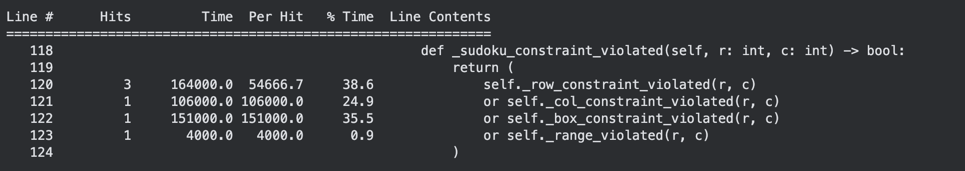
\includegraphics[width=\linewidth]{figures/line_profile2}
        \caption{The line profile of the \inlinecode{BacktrackingSolver._sudoku_constraint_violated} function. This indicates
        that no single line of code is responsible for the majority of the computation time, it is equally shared.}
        \label{fig:line_profile2}
    \end{subfigure}
    \hfill
    \begin{subfigure}[b]{0.9\linewidth}
        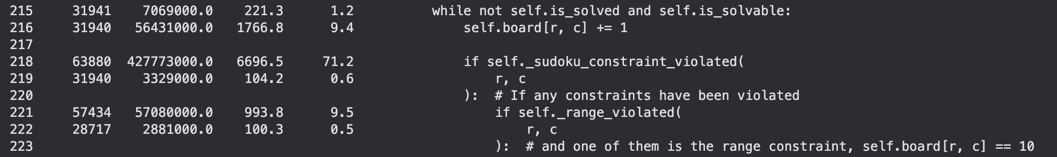
\includegraphics[width=\linewidth]{figures/line_profile3}
        \caption{The same line profile as in (a), but after optimisation. The key line here is line 218.}
        \label{fig:line_profile3}
    \end{subfigure}
    \caption{Line profiles of the \inlinecode{BacktrackingSolver.solve} function and the
    \inlinecode{BacktrackingSolver._sudoku_constraint_violated} functions. The headers of each column are shown in (b).
        (a), and (b) show the profiles before optimisation, and (c) shows a profile after optimisation.
        The key line in (a) and (c) is line 225 and 218 respectively, which show a 10.2x speedup after optimisation.}
    \label{fig:line_profile}
    \hfill
    \end{figure}
    Given that this was a very low requirement project, there was not much testing of third-party packages required.
    However, the performance of the code was tested using a line profiler.
    Fig.\eqref{fig:line_profile1} shows the line profile of the \inlinecode{BacktrackingSolver.solve} function before
    optimisation, which allowed us to identify the bottleneck of the code, where most of the time was being spent.
    This was useful as it allowed us to identify where to focus our optimisation efforts, and not waste time optimising
    code that was not responsible for the majority of the computation time.

    Given that \inlinecode{BacktrackingSolver._sudoku_constraint_violated} was the function that we identified as the
    bottleneck, the next steps was to optimise this function.
    Some options for this were re-write this function in Cython or C, or look into different algorithms or packages
    that could be used to implement this function.
    We decided to implement this function in C, by implementing a function \inlinecode{has_non_zero_duplicates} and made
    it executable in python using \inlinecode{ctypes}, a python standard library module.
    The functions called in lines 120 to 122 in Fig.\eqref{fig:line_profile2}, were then amended to use this new C function.
    This resulted in a 10.2x speedup of the \inlinecode{BacktrackingSolver.solve} function, as shown in Fig.\eqref{fig:line_profile3}.
    The raw speed-up from the implementation of \inlinecode{has_non_zero_duplicates} was closer to 20x but addition of
    error handling in the python wrapper reduced this to 10.2x.

    \subsection{Error handling}\label{subsec:coding-best-practises}
    General python best practises were followed with regard to error handling.
    Exceptions were raised when appropriate, and try except blocks were used to catch exceptions.
    Occasionally, a try except block was used to catch and re-raise exceptions (with no modification) for clarity.
    Likewise, try except blocks were used to catch potential errors, or invalid arguments to functions, and the in-built
    python exceptions were used to raise these errors to the user.
    The three most common exceptions that were raised were \inlinecode{ValueError}, \inlinecode{TypeError} and
    \inlinecode{FileNotFoundError}.
